\paragraph{В первой} главе рассмотрен алгоритм оценки параметров сигнала от одного источника в широкополосных системах связи на
фоне аддитивного гауссового  шума.

Схема алгоритма представлена на рисунке \ref{pic:ar_cdma1_scheme1}.

\begin{figure}[H]
	\center\scalebox{0.9}{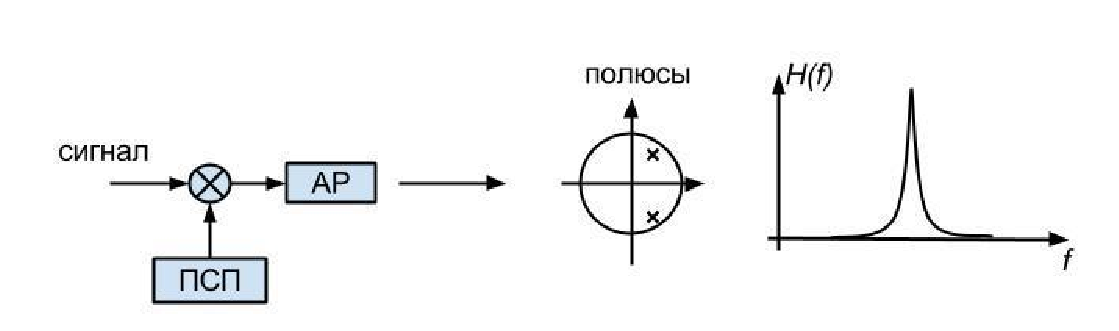
\includegraphics[width=1\linewidth]{lpc_for_1_sat_scheme.eps}}
	\caption{Детектирование сигнала АР-методом при известной фазе ПСП.}
	\label{pic:ar_cdma1_scheme1}
\end{figure}

Для восстановления гармонического сигнала из ШПС входная последовательность умножается на локально сформированную ПСП.
Далее запускается алгоритм на основе АР-модели. В реальных условиях приемник не имеет информации о фазе ПСП поэтому для детектирования
сигнала необходимо перебрать все возможные смещения расширяющего кода. Для ускорения вычислений предлагается использование алгоритма быстрого преобразования Фурье (БПФ).
Схема вычислений представлена на рисунке \ref{pic:ar_cdma1_scheme2}.

\begin{figure}[H]
	\center\scalebox{0.9}{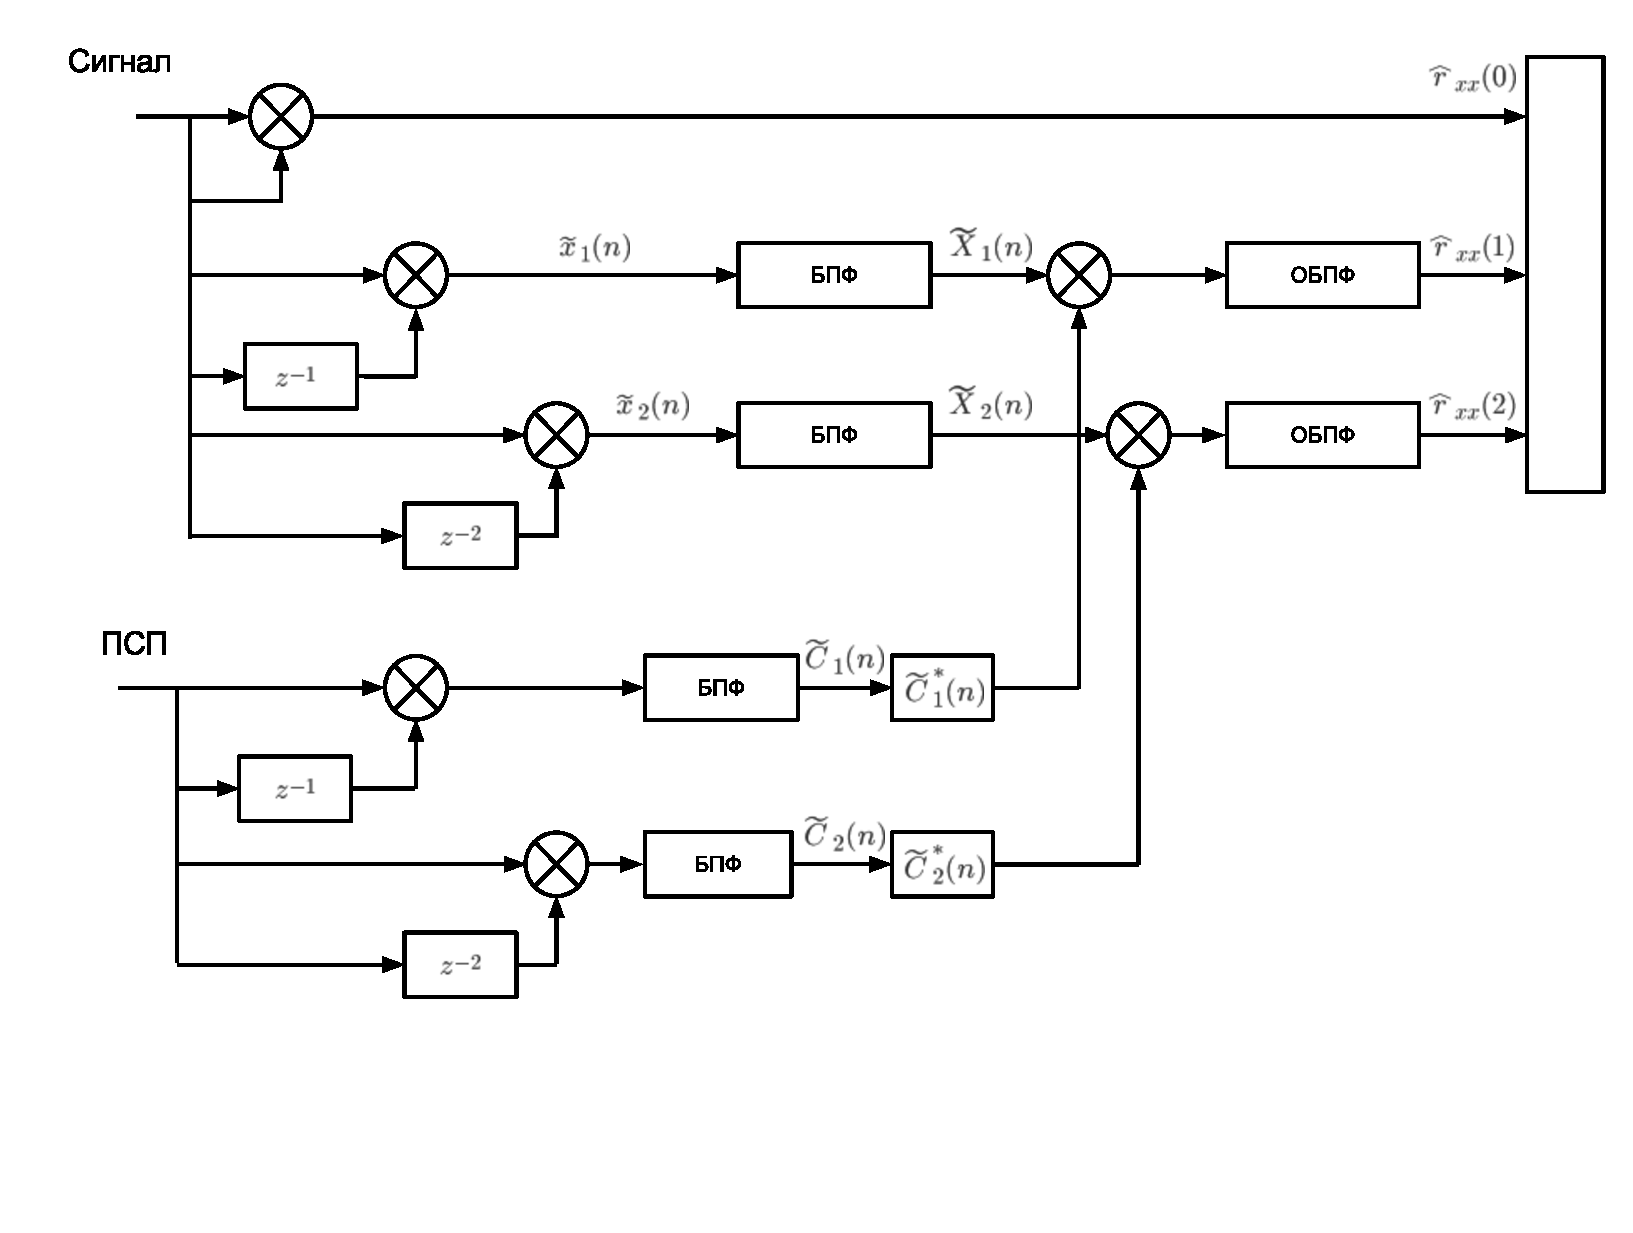
\includegraphics[width=1\linewidth]{lpc_fft.eps}}
	\caption{Общая схема применения АР модели для детектирования ШПС сигнала.}
	\label{pic:ar_cdma1_scheme2}
\end{figure}

Оценка ${\hat{r}_{xx}(0)}$ не зависит от выбранной фазы ПСП, поэтому она вычисляется один
раз для всех смещений кода. Далее формируется массив произведений входного сигнала на
свою задержанную копию ${\tilde{x}_1(n)=x(n)x(n-1)}$. Полученная последовательность  
${\tilde{x}_1(n)}$ поступает на вход алгоритма БПФ, в результате получаем массив ${\tilde{X}_1(n)}$
содержащий частотные отсчеты. Аналогично формируется массив  ${\tilde{X}_2(n)}$ для
задержки входного сигнала равной двум. Таким же способом обрабатываются локально
сгенерированные ПСП и формируются два массива ${\tilde{C}_1(n)}$ и ${\tilde{C}_2(n)}$.
Далее массивы ${\tilde{X}_1(n)}$ и ${\tilde{X}_1(n)}$ поэлементно перемножаются
на комплексно сопряженные массивы ${\tilde{C}_1^*(n)}$ и ${\tilde{C}_2^*(n)}$.
Результаты этих перемножений поступают на вход алгоритма обратного
БПФ. Полученные после ОБПФ два массива содержат оценки автокорреляционной функции для ${N}$ 
смещений кода, где  ${N}$ - размер данных на входе алгоритма БПФ.

Таким образом, предлагаемый алгоритм состоит из следующих шагов:

\begin{itemize}
\item[Шаг 1.] Вычисляются оценки  АКФ в трех первых точках (для аргументов АКФ=0,1,2)
	с использованием алгоритма БПФ для всех возможных смещений ПСП. 
\item[Шаг 2.] Для каждого смещения ПСП: 
	Определяются коэффициенты АР-модели ${\hat{a_1}, \hat{a_2}}$,
	вычисляется резонансная частота ${\omega_0}$
	и определяется квадрат модуля частотного отклика АР-модели для этой частоты. 
\item[Шаг 3.] Выбирается смещение ПСП для которого значение квадрата модуля частотного отклика было максимальным. Полученное значение сравнивается с заранее выбранным порогом детектора. 
	\subitem{\underline{Если}}  значение оказалось больше порогового {\underline{то}} 
		принимается решение о наличии сигнала, а в качестве оценки
		частоты принимается значение ${\omega_0}$ соответствующее выбранному смещению ПСП. 
	\subitem{\underline{Иначе}} 
		Принимается решение об отсутствии гармонического сигнала.
\end{itemize}

Разработанный алгоритм позволяет производить оценку частоты гармонического сигнала без использования прямого перебора как это делается в большинстве современных алгоритмов.
Например, алгоритм Delay and Multiply Approach (DMA) позволяет производить поиск только по смещению ПСП,
но он не дает возможности прямой оценки частоты. 
Предложенный алгоритм допускает сокращение количества операций умножения при переборе значений фазы ПСП за счет использования алгоритма БПФ.

Основным недостатком предложенного алгоритма является сильная чувствительность по отношению к интерференционным помехам: наличие «окрашенного» шума приводит к
значительному смещению получаемых оценок частоты и мощности гармонического сигнала.

Количество операций для оценки параметров от одного источника на фоне АБГШ:
\begin{center}
\begin{equation}
	%\label{}
	OP_{AR\_FOR\_1} = 24NlogN + 63N
\end{equation}
\end{center}

График вероятности оценки частоты в допустимом диапазоне входной расстройки представлен на рисунке
\ref{pic:lpc_for_1_probability}. Моделирование проводилось с аддитивным шумом, заданным в полосе от 0 Гц до
половины частоты дискретизации для одного, двух и трех шагов уточнения АКФ. В данном случае значение частоты дискретизации равно 16.368 МГц.
\begin{figure}[H]
\center\scalebox{1}{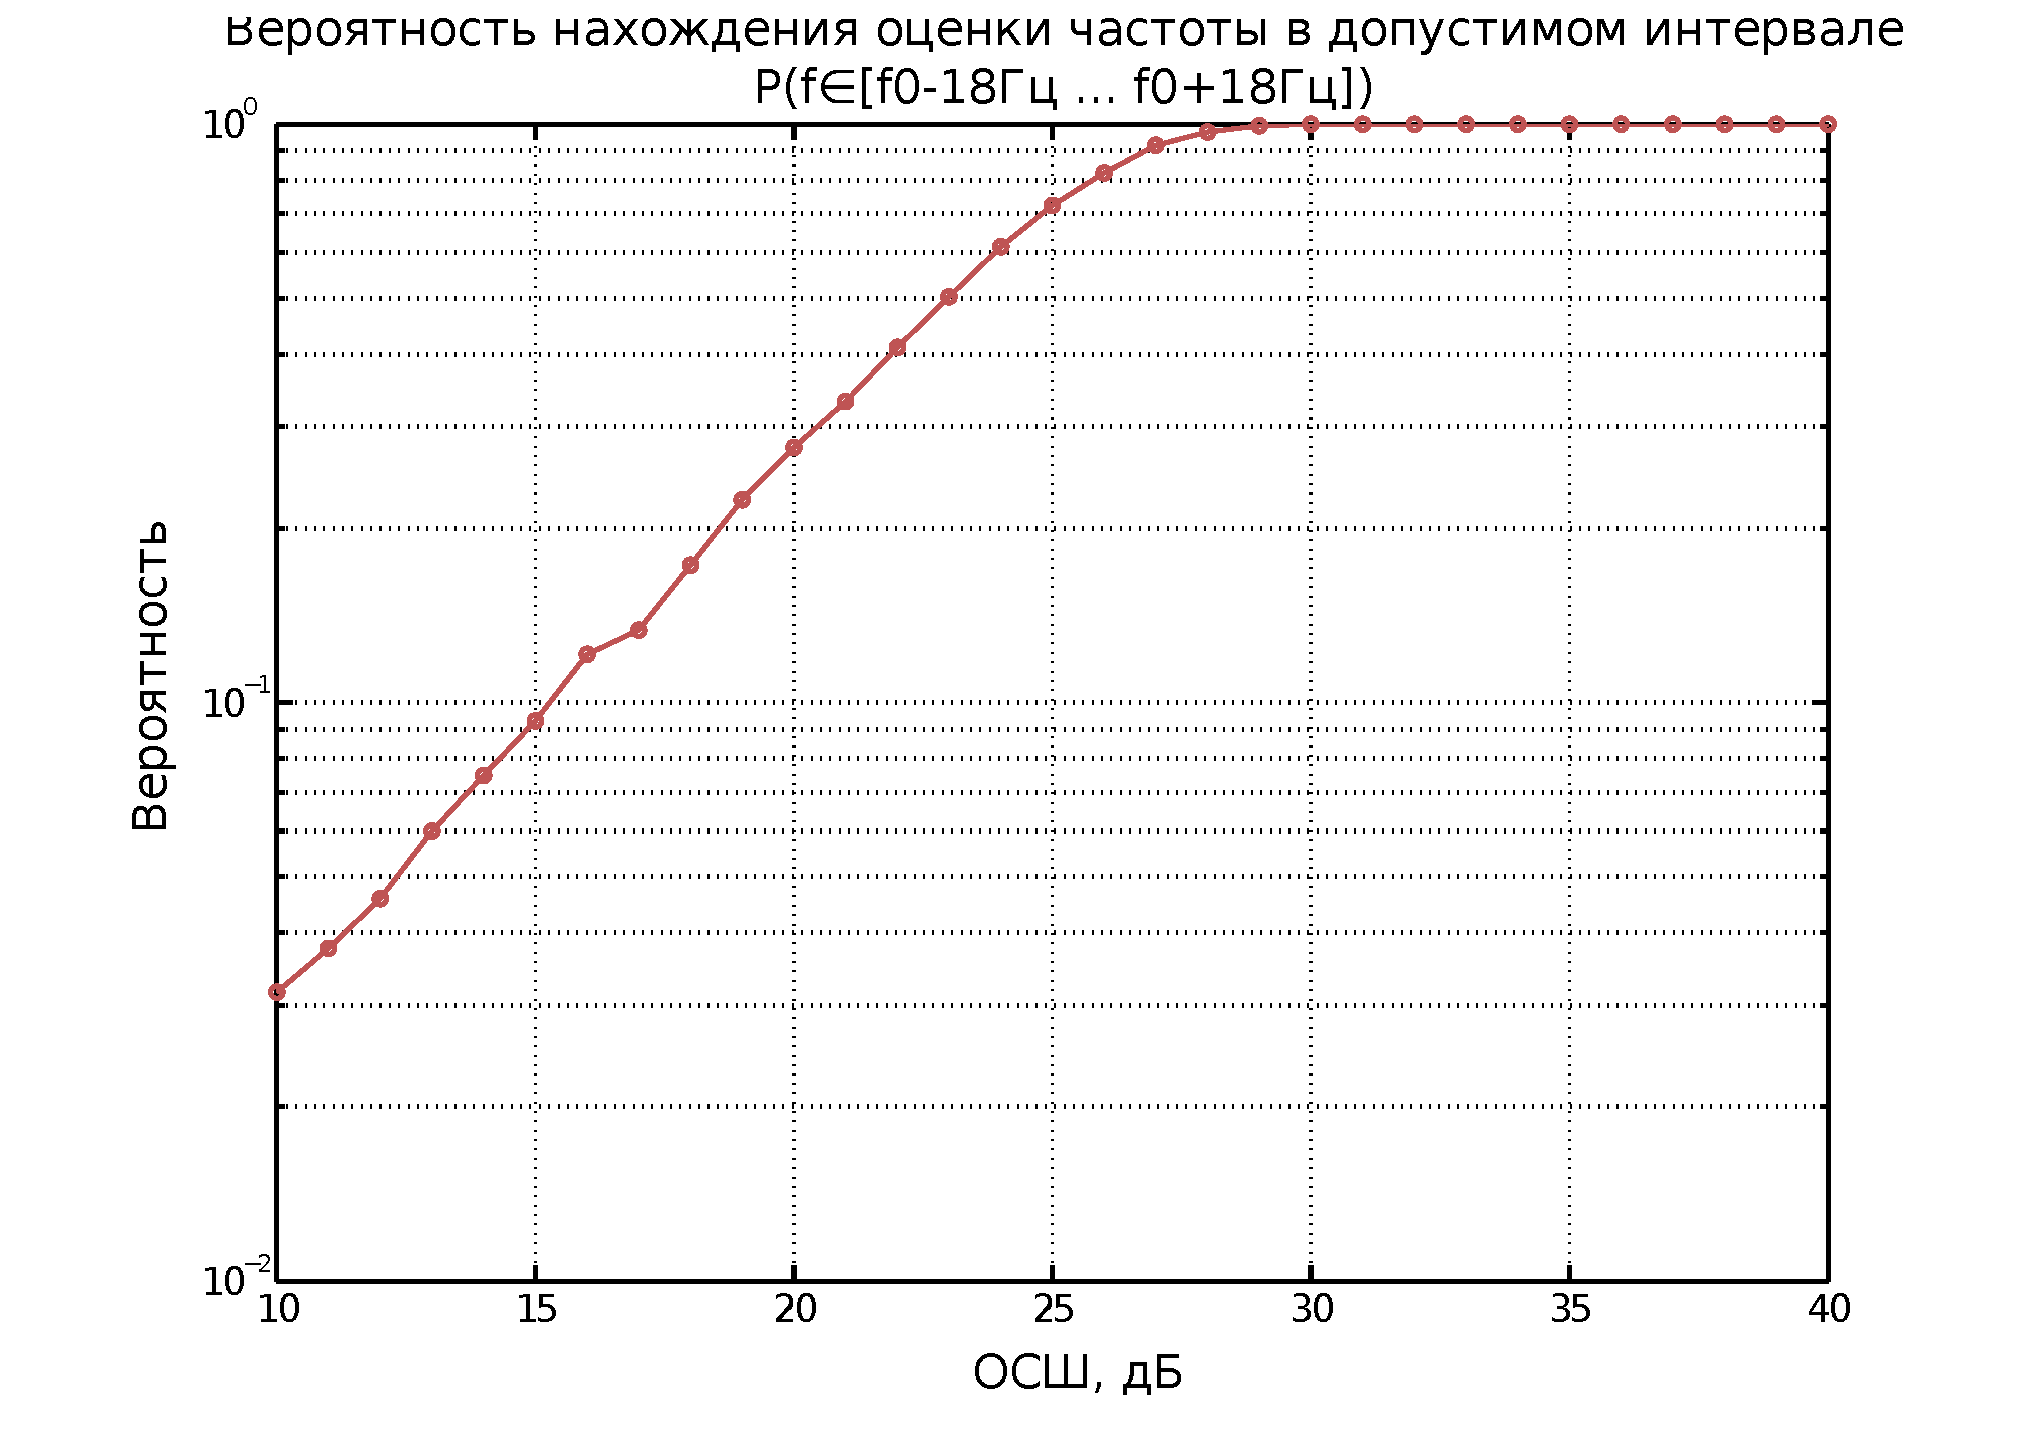
\includegraphics[width=1\linewidth]{lpc_for_1_probability.eps}}
	\caption{Вероятность оценки частоты удовлетворяющей допустимой входной расстройке}
	\label{pic:lpc_for_1_probability}
\end{figure}

Для оценки точности можно сравнить предлагаемый алгоритм с границей Крамера-Рао. Неравенство Крамера-Рао дает базу оценки, так
как представляет минимальную дисперсию среди всех классов оценщиков.
\begin{figure}[H]
\center\scalebox{1}{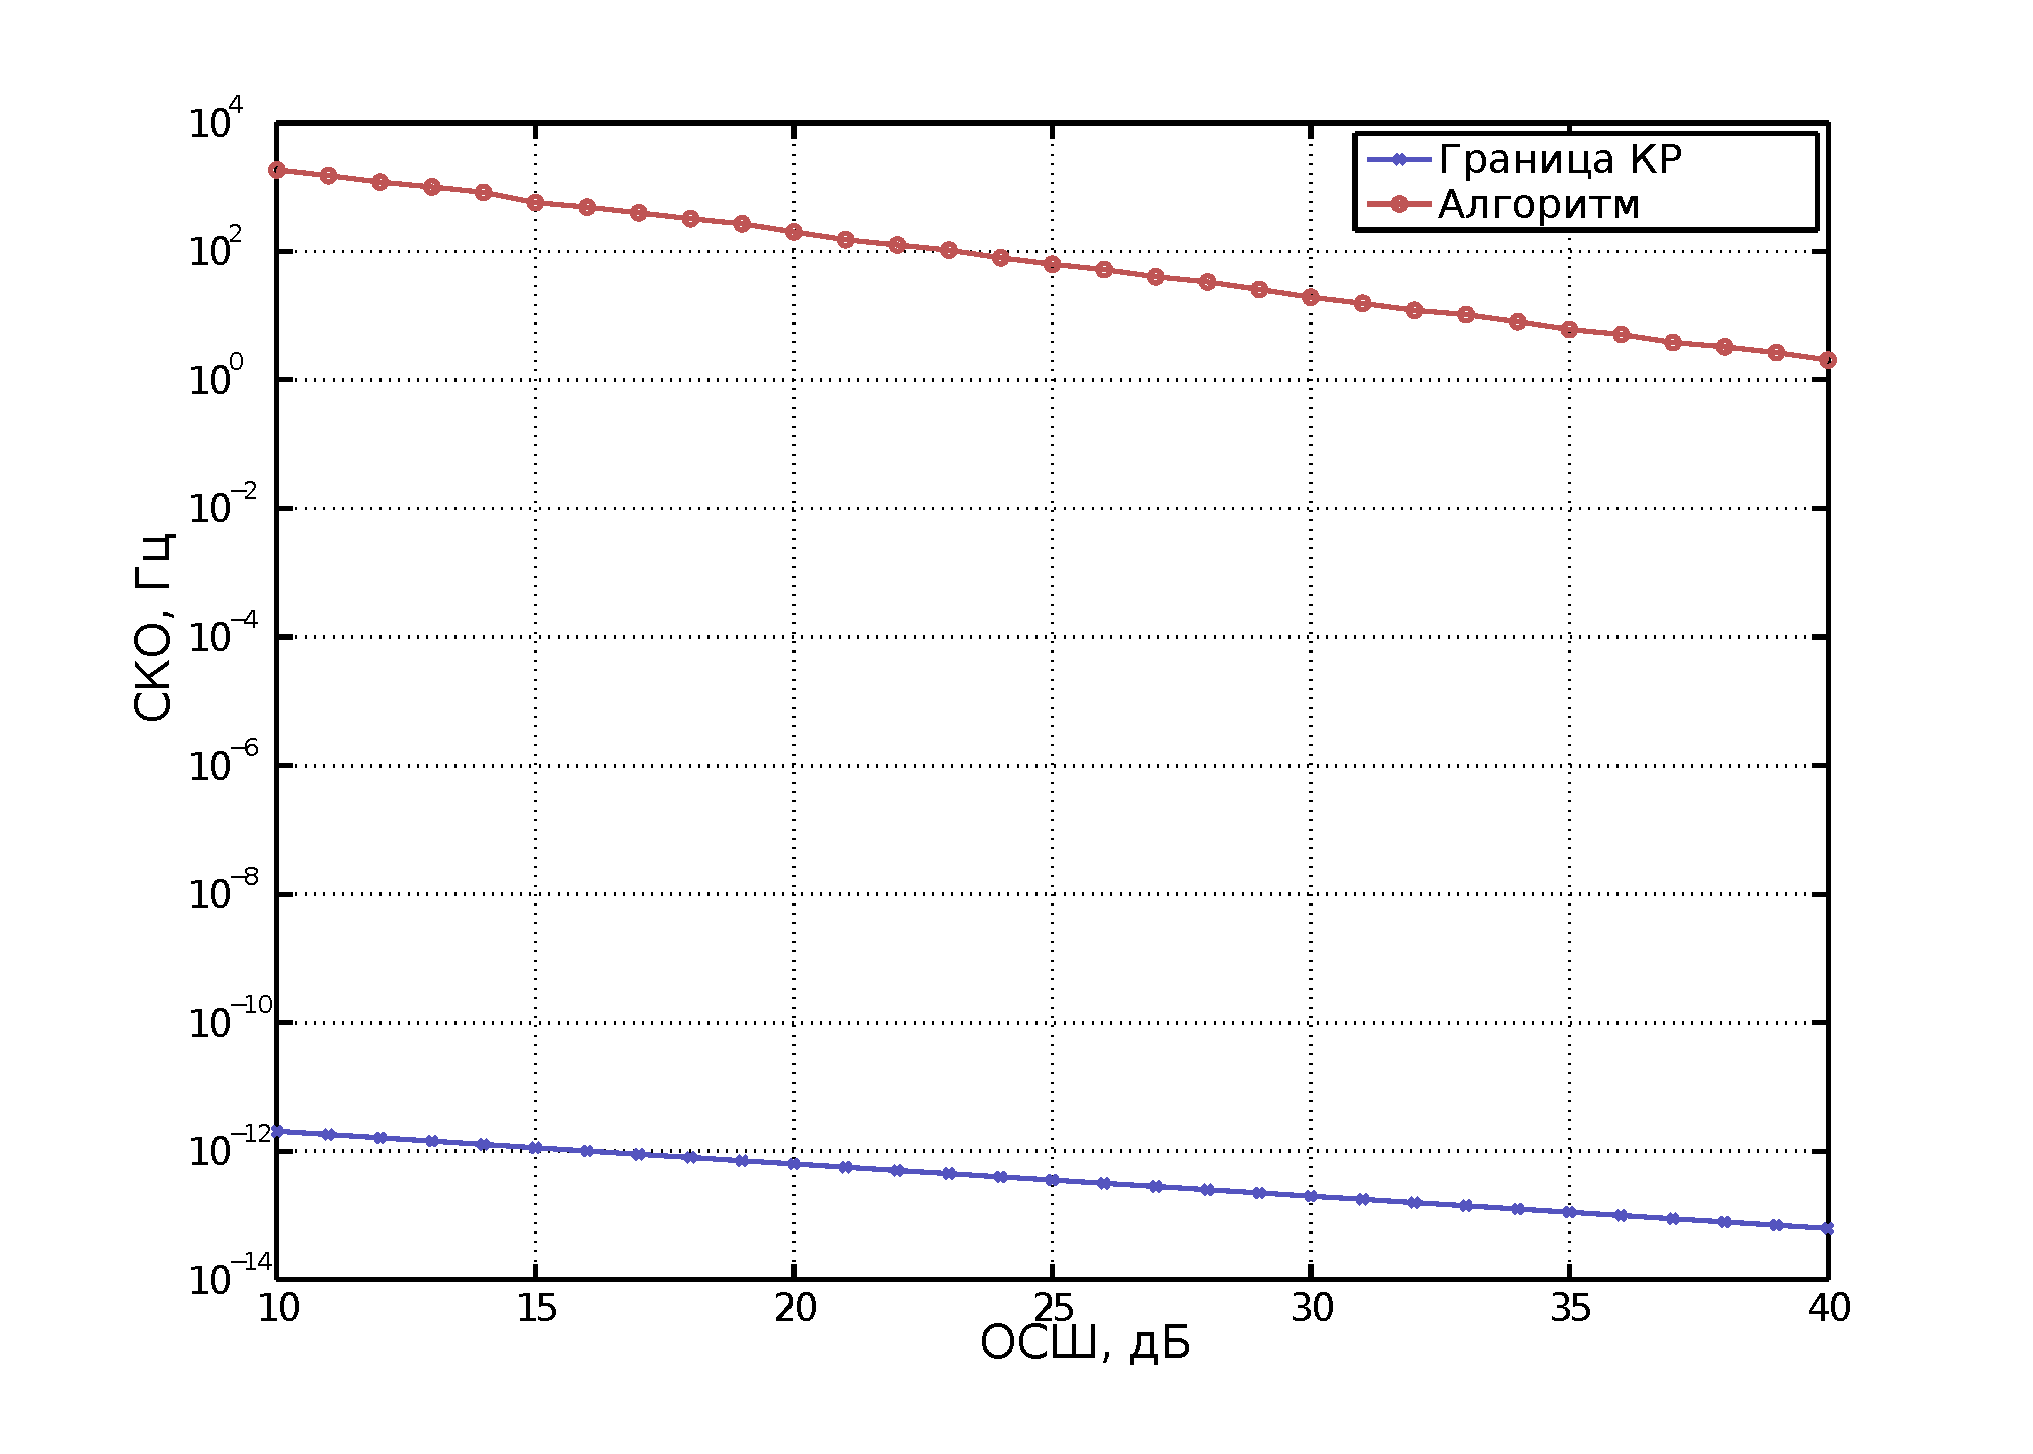
\includegraphics[width=1\linewidth]{crlb_vs_1sat_algo.eps}}
	\caption{СКО ошибка оценки частоты и граница Крамера-Рао в задаче оценки частоты гармонического сигнала}
	\label{pic:crlb_vs_1sat_algo}
\end{figure}
